
\de{ĐỀ THI HỌC KỲ I NĂM HỌC 2022-2023}{Trường THPT Lạc Long Quân - Bến Tre}

\begin{center}
	\textbf{PHẦN 1 - TRẮC NGHIỆM}
\end{center}
\Opensolutionfile{ans}[ans/ans]
\begin{ex}%[0D1Y1-5]%[Dự án đề kiểm tra HKI NH22-23- Võ Thị Thùy Trang]%[Lạc Long Quân-Bến Tre]
	Cho mệnh đề $P(x)\colon \exists x \in \mathbb{R}, x^2+3 x+4=0$. Mệnh đề phủ định của mệnh đề $P(x)$ là
	\choice
	{$\forall x \in \mathbb{R}, x^2+3 x+4=0$}
	{$\exists x \in \mathbb{R}, x^2+3 x+4 \neq 0$}
	{$\forall x \in \mathbb{R}, x^2+3 x+4>0$}
	{\True $\forall x \in \mathbb{R}, x^2+3 x+4 \neq 0$}
	\loigiai{Mệnh đề phủ định của mệnh đề $P(x)$ là $\forall x \in \mathbb{R}, x^2+3 x+4 \neq 0$.
	}
\end{ex}
\begin{ex}%[0D1B2-2]%[Dự án đề kiểm tra HKI NH22-23- Võ Thị Thùy Trang]%[Lạc Long Quân-Bến Tre]
	Tập hợp $S=\left\{x \in\mathbb{N}| x^2-4=0\right\}$ có số tập con là
	\choice
	{$3$}
	{$4$}
	{$1$}
	{\True $2$}
	\loigiai{Tập hợp $S=\left\{x \in\mathbb{N}| x^2-4=0\right\}=\{2\}$ có số tập con là $2$.
	}
\end{ex}
\begin{ex}%[0D1B3-2]%[Dự án đề kiểm tra HKI NH22-23- Võ Thị Thùy Trang]%[Lạc Long Quân-Bến Tre]
	Cho $A=\{x \in \mathbb{R}| x \leq 5\}$ và $B=\{x \in \mathbb{R}|-3<x \leq 10\}$. Khi đó tập hợp $\left(\mathrm{C}_R A\right)\setminus B$ bằng?
	\choice
	{$[5 ; 10]$}
	{\True $(10 ;+\infty)$}
	{$(-\infty ; 5)$}
	{$(-\infty ;-3)$}
	\loigiai{Ta có $\mathrm{C}_R A=\left(5;+\infty\right) \Rightarrow \left(\mathrm{C}_R A\right)\setminus B=\left(10;+\infty\right)$.
	}
\end{ex}
\begin{ex}%[0D2Y1-1]%[Dự án đề kiểm tra HKI NH22-23- Võ Thị Thùy Trang]%[Lạc Long Quân-Bến Tre]
	Cặp số $(2;-5)$ là nghiệm của bất phương trình nào sau đây?
	\choice
	{$x-2y \le 0$}
	{$3x-y<0$}
	{$2x+y<3$}
	{$x-3y<2$}
	\loigiai{Cặp số $(2;-5)$ là nghiệm của bất phương trình $2x+y<3$.
	}
\end{ex}
\begin{ex}%[0D2B1-1]%[Dự án đề kiểm tra HKI NH22-23- Võ Thị Thùy Trang]%[Lạc Long Quân-Bến Tre]
	Bạn Khoa để dành được một triệu đồng. Trong một đợt ủng hộ địa phương phòng chống Covid, Khoa đã lấy ra $x$ tờ tiền loại 20 nghìn đồng, $y$ tờ tiền loại 50 nghìn đồng để trao tặng. Một bất phương trình để mô tả điều kiện ràng buộc đối với $x$, $y$ là
	\choice
	{\True $20x+50y \le 1000$}
	{$20x+50y \ge 1000$}
	{$50x+20y \le 1000$}
	{$x+y \leq 1000$}
	\loigiai{Một bất phương trình để mô tả điều kiện ràng buộc đối với $x$, $y$ là $20x+50y \le 1000$.
	}
\end{ex}
\begin{ex}%[0D2B1-2]%[Dự án đề kiểm tra HKI NH22-23- Võ Thị Thùy Trang]%[Lạc Long Quân-Bến Tre]
 Miền nghiệm của bất phương trình $3x-2y>-6$ là miền nào dưới đây (miền không gạch sọc và không kể biên)?
	\choice
	{	\begin{tikzpicture}[scale=0.8,>=stealth, font=\footnotesize, line join=round, line cap=round]
			\def\xmin{-2} \def\xmax{2.5}
			\def\ymin{-1} \def\ymax{3.5}
			%\draw[color=gray!50,dashed] (\xmin,\ymin) grid (\xmax,\ymax);	
			\draw[->] (\xmin,0)--(\xmax,0) node [below]{$x$};
			\draw[->] (0,\ymin)--(0,\ymax) node [left]{$y$};
			\fill (0,0) circle (1pt) node[shift={(-135:3mm)}]{$O$};
			\clip (\xmin+0.1,\ymin+0.1) rectangle (\xmax-0.1,\ymax-0.1);
			\draw[smooth,samples=300] plot(\x,{-3/2*(\x)+3});
			\fill[pattern=north east lines,pattern color=blue,opacity=.7]plot[domain=\xmin:\xmax](\x,{\ymin})--plot[domain=\xmax:\xmin](\x,{-3/2*(\x)+3})--cycle;
			\fill (2,0) circle (1pt) node[shift={(70:3mm)}]{$2$};
			\fill (0,3) circle (1pt) node[shift={(20:3mm)}]{$3$};
	\end{tikzpicture}}
	{	\begin{tikzpicture}[scale=0.8,>=stealth, font=\footnotesize, line join=round, line cap=round]
			\def\xmin{-2.5} \def\xmax{2}
			\def\ymin{-1} \def\ymax{3.5}
			%\draw[color=gray!50,dashed] (\xmin,\ymin) grid (\xmax,\ymax);	
			\draw[->] (\xmin,0)--(\xmax,0) node [below]{$x$};
			\draw[->] (0,\ymin)--(0,\ymax) node [left]{$y$};
			\fill (0,0) circle (1pt) node[shift={(-135:3mm)}]{$O$};
			\clip (\xmin+0.1,\ymin+0.1) rectangle (\xmax-0.1,\ymax-0.1);
			\draw[smooth,samples=300] plot(\x,{3/2*(\x)+3});
			\fill[pattern=north east lines,pattern color=blue,opacity=.7]plot[domain=\xmin:\xmax](\x,{3/2*(\x)+3})--plot[domain=\xmax:\xmin](\x,{\ymin})--cycle;
			\fill (-2,0) circle (1pt) node[shift={(120:3mm)}]{$-2$};
			\fill (0,3) circle (1pt) node[shift={(-170:3mm)}]{$3$};
	\end{tikzpicture}}
	{\True \begin{tikzpicture}[scale=0.8,>=stealth, font=\footnotesize, line join=round, line cap=round]
			\def\xmin{-2.5} \def\xmax{2}
			\def\ymin{-1} \def\ymax{3.5}
			%\draw[color=gray!50,dashed] (\xmin,\ymin) grid (\xmax,\ymax);	
			\draw[->] (\xmin,0)--(\xmax,0) node [below]{$x$};
			\draw[->] (0,\ymin)--(0,\ymax) node [left]{$y$};
			\fill (0,0) circle (1pt) node[shift={(-135:3mm)}]{$O$};
			\clip (\xmin+0.1,\ymin+0.1) rectangle (\xmax-0.1,\ymax-0.1);
			\draw[smooth,samples=300] plot(\x,{3/2*(\x)+3});
			\fill[pattern=north east lines,pattern color=blue,opacity=.7]plot[domain=\xmin:\xmax](\x,{3/2*(\x)+3})--plot[domain=\xmax:\xmin](\x,{\ymax})--cycle;
			\fill (-2,0) circle (1pt) node[shift={(-40:3mm)}]{$-2$};
			\fill (0,3) circle (1pt) node[shift={(10:3mm)}]{$3$};
	\end{tikzpicture}}
	{	\begin{tikzpicture}[scale=0.8,>=stealth, font=\footnotesize, line join=round, line cap=round]
			\def\xmin{-2.5} \def\xmax{1.5}
			\def\ymin{-3.5} \def\ymax{1.5}
			%\draw[color=gray!50,dashed] (\xmin,\ymin) grid (\xmax,\ymax);	
			\draw[->] (\xmin,0)--(\xmax,0) node [below]{$x$};
			\draw[->] (0,\ymin)--(0,\ymax) node [left]{$y$};
			\fill (0,0) circle (1pt) node[shift={(-135:3mm)}]{$O$};
			\clip (\xmin+0.1,\ymin+0.1) rectangle (\xmax-0.1,\ymax-0.1);
			\draw[smooth,samples=300] plot(\x,{-3/2*(\x)-3});
			\fill[pattern=north east lines,pattern color=blue,opacity=.7]plot[domain=\xmin:\xmax](\x,{\ymin})--plot[domain=\xmax:\xmin](\x,{-3/2*(\x)-3})--cycle;
			\fill (-2,0) circle (1pt) node[shift={(70:3mm)}]{$-2$};
			\fill (0,-3) circle (1pt) node[shift={(20:3mm)}]{$-3$};
	\end{tikzpicture}}
	\loigiai{ Do đường thẳng $3x-2y-6$ đi qua hai điểm $(-2;0)$, $(0;3)$ và $3\cdot 0-2\cdot 0>-6$.
	}
\end{ex}
\begin{ex}%[0D3B1-2]%[Dự án đề kiểm tra HKI NH22-23- Võ Thị Thùy Trang]%[Lạc Long Quân-Bến Tre]
	Tập xác định của hàm số $y=\sqrt{5-3 x}$ là
	\choice
	{$\mathscr{D}=\left(-\infty ; \dfrac{5}{3}\right)$}
	{$\mathscr{D}=\mathbb{R} \setminus \left\{\dfrac{5}{3}\right\}$}
	{\True $\mathscr{D}=\left(-\infty ; \dfrac{5}{3}\right]$}
	{$\mathscr{D}=\left[\dfrac{5}{3} ;+\infty\right)$}
	\loigiai{Hàm số $y=\sqrt{5-3 x}$ xác định khi và chỉ khi $5-3x\ge 0  \Leftrightarrow x\le \dfrac{5}{3}$.\\
		Vậy tập xác định của hàm số là $\mathscr{D}=\left( -\infty;\dfrac{5}{3}\right]$.
	}
\end{ex}
\begin{ex}%[0D3B2-3]%[Dự án đề kiểm tra HKI NH22-23- Võ Thị Thùy Trang]%[Lạc Long Quân-Bến Tre]
	\immini{
		Đồ thị bên là của hàm số nào?
	\choice
	{$y=-x^2+2x-3$}
	{\True $y=-x^2+2 x+3$}
	{$y=x^2+2 x-3$}
	{$y=-x^2+2 x+4$}}
	{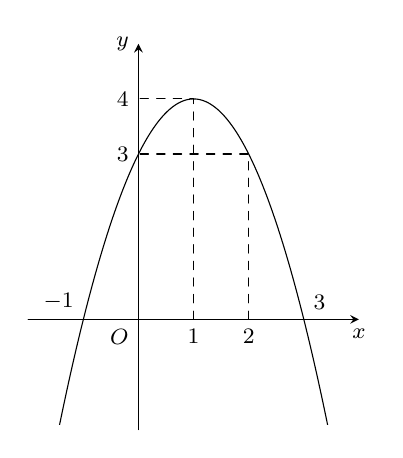
\begin{tikzpicture}[scale=.7,>=stealth, font=\footnotesize, line join=round, line cap=round]
			\def\a{-1} \def\b{2} \def\c{3} % Hệ số
			\def\xmin{-2} \def\xmax{4}
			\def\ymin{-2} \def\ymax{5}
			\draw[->] (\xmin,0)--(\xmax,0) node [below]{$x$};
			\draw[->] (0,\ymin)--(0,\ymax) node [left]{$y$};
			\node at (0,0) [below left]{$O$};
			\draw[dashed] (1,0)node [below]{$1$}--(1,4)--(0,4)node [left]{$4$} ;
			\draw[dashed] (2,0)node [below]{$2$}--(2,3)--(0,3)node [left]{$3$};
			\node at (-1,0)[above left]{$-1$};
			\node at (3,0)[above right]{$3$};
			\clip (\xmin+0.1,\ymin+0.1) rectangle (\xmax-0.5,\ymax-0.1);
			\draw[smooth,samples=300] plot(\x,{\a*(\x)^2+\b*(\x)+\c});
	\end{tikzpicture}}
	\loigiai{Do $x=0 \Rightarrow y=3$ nên ta chọn $y=-x^2+2 x+3$.
	}
\end{ex}
\begin{ex}%[0H1B1-2]%[Dự án đề kiểm tra HKI NH22-23- Võ Thị Thùy Trang]%[Lạc Long Quân-Bến Tre]
Trong tam giác $ABC$ biết số đo $A=85^{\circ} 35^{\prime}$ ; $B=79^{\circ} 25^{\prime}$. Giá trị của $\sin C$ là
	\choice
	{\True $\sin C=\dfrac{\sqrt{6}-\sqrt{2}}{4}$}
	{$\sin C=\dfrac{\sqrt{6}+\sqrt{2}}{4}$}
	{$\sin C=1$}
	{$\sin C=15^{\circ}$}
	\loigiai{Ta có $\sin C=\sin \left(180^\circ-\left(85^{\circ} 35^{\prime}+79^{\circ} 25^{\prime}\right)\right)=\sin 15^\circ=\dfrac{\sqrt{6}-\sqrt{2}}{4}$.
	}
\end{ex}
\begin{ex}%[0H1Y2-2]%[Dự án đề kiểm tra HKI NH22-23- Võ Thị Thùy Trang]%[Lạc Long Quân-Bến Tre]
	Tính diện tích $S$ của tam giác $ABC$ có độ dài $a=5$ cm, $c=8$ cm và số đo góc $B=120^{\circ}$.
	\choice
	{$S=20\sqrt{3} \mathrm{~cm}^2$}
	{$S=20 \mathrm{~cm}^2$}
	{$S=10 \mathrm{~cm}^2$}
	{\True $S=10 \sqrt{3} \mathrm{~cm}^2$}
	\loigiai{Ta có $S=\dfrac{1}{2}\cdot a\cdot c\cdot \sin B=\dfrac{1}{2}\cdot 5\cdot 8\cdot \sin 120^\circ=10 \sqrt{3} \mathrm{~cm}^2$.
	}
\end{ex}
\begin{ex}%[0H1B2-1]%[Dự án đề kiểm tra HKI NH22-23- Võ Thị Thùy Trang]%[Lạc Long Quân-Bến Tre]
		Cho tam giác $ABC$ có $B=65^{\circ}$ và độ dài $b=12$. Bán kính $R$ của đường tròn ngoại tiếp tam giác $ABC$ là (kết quả làm tròn đến hai chữ số thập phân)
	\choice
	{\True $R=6{,}62$}
	{$R=13{,}24$}
	{$R=28{,}39$}
	{$R=14{,}20$}
	\loigiai{Ta có $R=\dfrac{b}{2\sin B}=\dfrac{12}{2\sin 65^\circ}\approx 6{,}62$.
	}
\end{ex}
\begin{ex}%[0H1K2-1]%[Dự án đề kiểm tra HKI NH22-23- Võ Thị Thùy Trang]%[Lạc Long Quân-Bến Tre]
	\immini{Biết từ một điểm cách hai đầu của một hồ nước lần lượt là $800$ m và $900$ m  người quan sát nhìn hai điểm này dưới một góc $70^{\circ}$ (như hình vẽ). Khoảng cách giữa hai điểm ở hai đầu của hồ nước gần với kết quả nào nhất?
		\choice
		{$900$ m}
		{\True $979$ m}
		{$312$ m}
		{$1098$ m}	}
	{\definecolor{ecru}{rgb}{0.76, 0.7, 0.5}
		\definecolor{lightcornflowerblue}{rgb}{0.6, 0.81, 0.93}
		\definecolor{brightpink}{rgb}{1.0, 0.0, 0.5}
		\definecolor{ashgrey}{rgb}{0.7, 0.75, 0.71}
		
		\definecolor{green(ryb)}{rgb}{0.4, 0.69, 0.2}
		\definecolor{dollarbill}{rgb}{0.52, 0.73, 0.4}
		\definecolor{deepskyblue}{rgb}{0.0, 0.75, 1.0}
		\begin{tikzpicture}[line join=round, line cap=round,scale=.5,transform shape]
			\clip (-6,-6.5) rectangle (6,2);
			
			
			\tikzset{ho/.pic={
					\def\D{ 
						(-6,-.7)
						..controls +(5:1.5) and +(-170:.7) ..(.8,-1.1)
						..controls +(10:1.2) and +(170:.7) ..(6,-.6)--(6,-6.5)--(-6,-6.5)--cycle
						;
					}
					\draw[green(ryb)]\D;
					\fill[green(ryb)] \D;
					
					\def\D1{ 
						(-6,-1.2)
						..controls +(5:1.5) and +(-170:.7) ..(.8,-1.15)
						..controls +(10:1.2) and +(170:.5) ..(6,-1.2)--(6,-6.5)--(-6,-6.5)--cycle
						;
					}
					\draw[dollarbill]\D1;
					\fill[dollarbill] \D1;
					
					\def\T{ 
						(-6,-.7)
						..controls +(5:1.5) and +(-170:.7) ..(.8,-1.1)
						..controls +(10:1.2) and +(170:.7) ..(6,-.6)--(6,3)--(-6,3)--cycle
						;
					}
					\draw[ecru!70!black]\T;
					\fill[bottom color=white,top color=deepskyblue!90, middle color=white] \T;
					
					\def\D1{ 
						(.58,-1.35)
						..controls +(0:.3) and +(-10:.3) ..(.55,-1.15)
						..controls +(175:.1) and +(95:.3) ..(0,-1.3)--cycle
						
						(-.55,-1.28)
						..controls +(0:.1) and +(-10:.1) ..(-.58,-1.1)
						..controls +(175:.1) and +(15:.3) ..(-.85,-1.15)
						..controls +(-135:.1) and +(170:.1) ..(-.8,-1.3)
						;
					}
					\draw[ashgrey]\D1;
					\fill[ashgrey!60] \D1;
					
					\def\H{ 
						(0,-1.3)
						..controls +(175:1) and +(-5:.7) ..(-2,-1.4)
						..controls +(-175:.4) and +(85:.3) ..(-2.7,-1.6)
						..controls +(-95:.2) and +(65:.2) ..(-3.9,-1.7)
						..controls +(-115:.2) and +(-170:.3) ..(-2,-1.85)
						..controls +(-170:.2) and +(180:.5) ..(-2,-2)
						..controls +(0:1) and +(-170:2) ..(2,-1.95)
						..controls +(-170:.2) and +(175:.5) ..(3.5,-1.85)
						..controls +(-5:.8) and +(0:.5) ..(3.7,-1.65)
						..controls +(180:1) and +(-10:.5) ..(2.5,-1.4)
						..controls +(170:1) and +(-10:.5) ..cycle
						;
					}
					\draw[green(ryb)]\H;
					\fill[lightcornflowerblue] \H;
					
					\def\D3{ 
						(3,-2)
						..controls +(55:.2) and +(-20:.2) ..(3,-1.7)
						..controls +(175:.2) and +(95:.1) ..(2.5,-1.8)
						..controls +(-175:.1) and +(85:.3) ..(2.1,-2)
						..controls +(-95:.1) and +(-125:.1) ..cycle
						;
					}
					\draw[ashgrey]\D3;
					\fill[ashgrey!60] \D3;
					
			}}
			
			
			\tikzset{co/.pic={
					\def\C{ 
						(-3.6,-3)
						..controls +(85:.05) and +(-30:.1) ..(-3.75,-2.85)
						(-3.6,-3)
						..controls +(85:.05) and +(-30:.1) ..(-3.7,-2.75)
						(-3.6,-3)
						..controls +(80:.05) and +(-160:.1) ..(-3.5,-2.9)
						(-3.6,-3)
						..controls +(80:.05) and +(-160:.1) ..(-3.45,-2.7)
						;
					}
					\draw[green(ryb)] \C;
					%\fill[green(ryb)] \C;
			}}
			
			\tikzset{hoa/.pic={
					\def\H{
						(0,0)
						..controls +(0:2) and +(60:2) .. (0,0)
						..controls +(60:2) and +(120:2) .. (0,0)
						..controls +(120:2) and +(180:2) .. (0,0)
						..controls +(180:2) and +(240:2) .. (0,0)
						..controls +(240:2) and +(300:2) .. (0,0)
						..controls +(300:2) and +(360:2) .. (0,0)
						;}
					\fill[brightpink] \H;
					%\draw[brightpink] \H;
			}}
			
			\path
			(0,0)pic[scale=1]{ho}
			(0,0)pic[scale=1]{co} (.2,0)pic[scale=1]{co}
			(.3,0)pic[scale=1]{co} (.4,.1)pic[scale=1]{co}
			(.5,.3)pic[scale=1]{co} (.6,0)pic[scale=1]{co}
			(.7,0)pic[scale=1]{co} (.8,.2)pic[scale=1]{co}
			(2,0)pic[scale=1]{co} (2.2,0)pic[scale=1]{co}
			(2.3,0)pic[scale=1]{co} (2.1,.1)pic[scale=1]{co}
			(7,1)pic[scale=1]{co} (7.2,1)pic[scale=1]{co}
			(7.3,1)pic[scale=1]{co} (7.1,1.1)pic[scale=1]{co}
			(5.6,.85)pic[scale=1]{co} (5.8,.9)pic[scale=1]{co}
			(7.1,-1.2)pic[scale=1]{co} (7.2,-1)pic[scale=1]{co}
			(7.8,-1)pic[scale=1]{co} (7.6,-1.2)pic[scale=1]{co}
			(7.7,-1.3)pic[scale=1]{co} (7.5,-1.1)pic[scale=1]{co}
			(7,-1.1)pic[scale=1]{co} (7.3,-1.2)pic[scale=1]{co}
			(-3.5,-2.5)pic[scale=.07]{hoa} (-3.3,-2.6)pic[scale=.07]{hoa} (-2.8,-2.4)pic[scale=.07]{hoa}
			(3.5,-3.7)pic[scale=.07]{hoa} (4.3,-4.1)pic[scale=.07]{hoa}
			(3.8,-3.6)pic[scale=.07]{hoa} (-1.5,-2.6)pic[scale=.07]{hoa} (3.75,-3.8)pic[scale=.07]{hoa} (4,-3.7)pic[scale=.07]{hoa};
			
			\path 	(1,-6.3) coordinate (A)
			(-3.9,-1.75) coordinate (B)
			(4.1,-1.75) coordinate (C)
			;
			\draw (C)--(A)--(B);
			\draw[dashed] (B)--(C);
			\node at (-2.5,-4.5) [right]{\large $800$ m};
			\node at (2.4,-4.5) [right]{\large $900$ m};
			%\foreach \x/\g in {A/-90,B/180,C/0} \fill (\x) circle (1.5pt)+(\g:3mm) node {$\x$};
			\draw pic["\large $70^\circ$", draw=black, angle eccentricity=2,angle radius=.3cm, color=black]
			{angle=C--A--B};
	\end{tikzpicture}} 
	\loigiai{ Khoảng cách giữa hai điểm ở hai đầu của hồ nước là $$\sqrt{800^2+900^2-2\cdot 800\cdot 900\cdot \cos 70^\circ}\approx 979~ \mathrm{m}.$$ 
	}
\end{ex}
	\begin{ex}%%[0H2B1-2]%[Dự án đề kiểm tra HKI NH22-23- Võ Thị Thùy Trang]%[Lạc Long Quân-Bến Tre]
    \immini{Cho hình lục giác đều $ABCDEF$. Có bao nhiêu véc-tơ cùng hướng với $\overrightarrow{AB}$.
    	\choice
    	{$5$}
    	{$7$}
    	{$3$}
    	{\True $4$}
    }	
{	\begin{tikzpicture}[scale=0.7,>=stealth, font=\footnotesize, line join=round, line cap=round]
		\def\a{3}
		\path (0:0) coordinate (O)
		++(180:\a) coordinate (A) 
		([turn]120:\a) coordinate (B)
		++(0:\a) coordinate (C)
		++(60:\a) coordinate (D)
		++(120:\a) coordinate (E)
		++(180:\a) coordinate (F)
		;
		\draw (A)--(B)--(C)--(D)--(E)--(F)--cycle;
		\draw (F)--(C) (E)--(B) (A)--(D);
		\foreach \x/ \goc in {A/135,O/90,B/-45,C/0,D/0,E/0,F/90} 
		\fill (\x) circle (1pt)
		($(\x)+(\goc:3mm)$) node {$\x$}; 
\end{tikzpicture}}
	\loigiai{ Các véc-tơ cùng hướng với $\overrightarrow{AB}$ là $\overrightarrow{FO}$, $\overrightarrow{OC}$, $\overrightarrow{ED}$, $\overrightarrow{FC}$.
	}
\end{ex}
\begin{ex}%[0H2B4-2]%[Dự án đề kiểm tra HKI NH22-23- Võ Thị Thùy Trang]%[Lạc Long Quân-Bến Tre]
	Tính góc $(\overrightarrow{a}, \overrightarrow{b})$ biết $2\overrightarrow{a} \cdot \overrightarrow{b}=-\sqrt{3}\cdot\left|\overrightarrow{a}\right|\cdot\left|\overrightarrow{b}\right|$, $(\overrightarrow{a}, \overrightarrow{b} \neq \overrightarrow{0})$
	\choice
	{$120^\circ$}
	{$135^\circ$}
	{\True $150^\circ$}
	{$60^\circ$}
	\loigiai{Ta có $\cos (\overrightarrow{a}, \overrightarrow{b})=\dfrac{\overrightarrow{a} \cdot \overrightarrow{b}}{\left|\overrightarrow{a}\right|\cdot\left|\overrightarrow{b}\right|}=\dfrac{-\sqrt{3}}{2} \Rightarrow  (\overrightarrow{a}, \overrightarrow{b})=150^\circ$.
	}
\end{ex}

\begin{ex}%[0D1B1-3]%[Dự án đề kiểm tra HKI NH22-23- Võ Thị Thùy Trang]%[Lạc Long Quân-Bến Tre]
	Số quy tròn của số $205454$ với độ chính xác $d=100$ là
	\choice
	{\True $205000$}
	{$205400$}
	{$205500$}
	{$206000$}
	\loigiai{Số quy tròn của số $205454$ với độ chính xác $d=100$ là $205000$.
	}
\end{ex}
\begin{ex}%[0D1B4-3]%[Dự án đề kiểm tra HKI NH22-23- Võ Thị Thùy Trang]%[Lạc Long Quân-Bến Tre]
	Phương sai của dãy số liệu $5$; $7$; $10$; $8$; $5$; $1$; $4$ là (kết quả làm tròn đến hai chữ số thập phân)
	\choice
	{$4{,}25$}
	{$8{,}5$}
	{$3{,}25$}
	{\True $7{,}35$}
	\loigiai{Ta có $\overline{x}=\dfrac{5+7+10+8+5+1+4}{7}=\dfrac{40}{7}$.\\
		Phương sai $S^2=\dfrac{1}{7}\left[\left(5-\dfrac{40}{7}\right)^2+\left(7-\dfrac{40}{7}\right)^2+\left(10-\dfrac{40}{7}\right)^2\right]$\\
		$+\dfrac{1}{7}\left[\left(8-\dfrac{40}{7}\right)^2+\left(5-\dfrac{40}{7}\right)^2+\left(1-\dfrac{40}{7}\right)^2+\left(4-\dfrac{40}{7}\right)^2\right]\approx 7{,}35$.
	}
\end{ex}
\Closesolutionfile{ans}

\begin{center}
	\textbf{PHẦN 2 - TỰ LUẬN}
\end{center}
\begin{bt}%[0H2B2-5]%[Dự án đề kiểm tra HKI NH22-23- Tên Huỳnh Quy]%[THPT Lạc Long Quân - Bến Tre]
	Cho tam giác $ABC$ vuông tại $A$ có độ dài $AB=5$, $AC=5\sqrt{3}$. Tính độ dài $\left|\vec{AC}-\vec{AB}\right|$.
	\loigiai{
	Ta có $\left|\vec{AC}-\vec{AB}\right|=|\vec{BC}|=BC=\sqrt{AB^2+AC^2}=\sqrt{5^2+\left(5\sqrt{3}\right)^2}=10$.	
}
\end{bt}

\begin{bt}%[0H2B4-1]%[Dự án đề kiểm tra HKI NH22-23- Tên Huỳnh Quy]%[THPT Lạc Long Quân - Bến Tre]
	Cho hình vuông $ABCD$ và có độ dài $AB=a$. Tính tích vô hướng $\vec{CA}\cdot\vec{AD}$.
	\loigiai{	
	\immini{Ta có
		\begin{eqnarray*}
		&&\vec{CA}\cdot\vec{AD}\\
		&=&|\vec{CA}|\cdot|\vec{AD}|\cdot\cos\left(\vec{CA},\vec{AD}\right)\\
		&=&a\sqrt{2}\cdot a\cdot\cos135^{\circ}\\
		&=&-a^2.	
		\end{eqnarray*} }{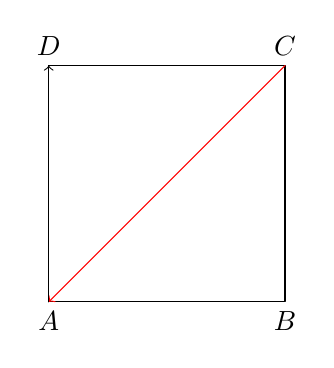
\begin{tikzpicture}[scale=1, line join=round, line cap=round]
			\def\a{3}
			\draw (0,0)--(\a,0)--(\a,\a)--(0,\a)--cycle;	
			\draw[->,red] (\a,\a)--(0,0);
			\draw[->](0,0)--(0,\a);
			\draw (0,0) node[below]{$A$};
			\draw (\a,0) node[below]{$B$};
			\draw (\a,\a) node[above]{$C$};
			\draw (0,\a) node[above]{$D$};
	\end{tikzpicture}}
	}
\end{bt}

\begin{bt}%[0D1B3-3]%[Dự án đề kiểm tra HKI NH22-23- Tên Huỳnh Quy]%[THPT Lạc Long Quân - Bến Tre]
	Hãy tìm khoảng biến thiên, số trung bình, trung vị, khoảng tứ phân phân vị của mẫu số liệu sau: $13$; $15$; $12$; $10$; $13$; $13$; $15$; $29$; $17$; $20$; $18$.
	\loigiai{
	Sắp xếp lại các số liệu theo thứ tự không giảm, ta được: $10$; $12$; $13$; $13$; $13$; $15$; $15$; $17$; $18$; $20$; $29$.
	\begin{itemize}
		\item Khoảng biến thiên: $R=29-10=19$.
		\item Số trung bình: $\overline{x}=\dfrac{175}{11}\approx 15{,}91$ (có thể lấy kết quả làm tròn).
		\item Trung vị: $M_e=15$.
		\item Tứ phân vị: $Q_1=13$; $Q_2=15$; $Q_3=18$.
		\item Khoảng tứ phân vị: $\Delta_Q=Q_3-Q_1=18-13=5$.
	\end{itemize}	
	}
\end{bt}
\begin{bt}%[0D3B2-3]%[Dự án đề kiểm tra HKI NH22-23- Tên Huỳnh Quy]%[THPT Lạc Long Quân - Bến Tre]
	Lập bảng biến thiên và vẽ đồ thị hàm số $y=-x^2+4x-3$.
	\loigiai{
		Tọa độ đỉnh $S(2;1)$.\\
		Trục đối xứng: $x=2$.\\
		Hệ số $a=-1<0$ nên bề lõm quay xuống.\\
		Bảng biến thiên:
		\begin{center}
			
\begin{tikzpicture}
				\tkzTabInit[lgt=1.2,espcl=4]
				{$x$/1,$f(x)$/2}
				{$-\infty$,$2$,$+\infty$}
				\tkzTabVar{-/$-\infty$,+/$1$,-/$-\infty$}
			\end{tikzpicture}
		\end{center}
	Bảng giá trị:
	\begin{center}
		\begin{tabular}{|c|c|c|c|c|c|}\hline
			{$x$}&{$0$}&{$1$}&{$2$}&{$3$}&{$4$}\\\hline
			{$y$}&{$-3$}&{$0$}&{$1$}&{$0$}&{$-3$}\\ \hline
		\end{tabular}
	\end{center}
	Đồ thị:
		\begin{center}
			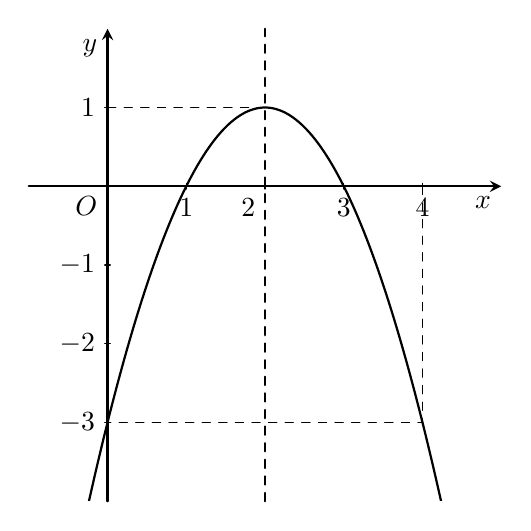
\begin{tikzpicture}[line join=round, line cap=round,>=stealth,thick]
				\tikzset{label style/.style={font=\footnotesize}}
				%%Nhập giới hạn đồ thị và hàm số cần vẽ
				\def \xmin{-1}
				\def \xmax{5}
				\def \ymin{-4}
				\def \ymax{2}
				\def \hamso{-(\x)^2+4*(\x)-3}
				%\def \tiemcanxien{\x+1}
				%%Tự động
				\draw[->] (\xmin,0)--(\xmax,0) node[below left] {$x$};
				\draw[->] (0,\ymin)--(0,\ymax) node[below left] {$y$};
				\draw (0,0) node [below left] {$O$};
				%%Vẽ các điểm trên 2 hệ trục
				\foreach \x in {1,3,4}
				\draw[thin] (\x,1pt)--(\x,-1pt) node [below] {$\x$};
				\foreach \x in {2}
				\draw[thin] (\x,1pt)--(\x,-1pt) node [below left] {$\x$};
				\foreach \y in {-3,-2,-1,1}
				\draw[thin] (1pt,\y)--(-1pt,\y) node [left] {$\y$};
				%%Vẽ thêm mấy cái râu ria
				\draw[dashed,thin](0,1)--(2,1);
				\draw[dashed,thin](4,0)--(4,-3)--(0,-3);
				%%Tự động
				\begin{scope}
					\clip (\xmin+0.01,\ymin+0.01) rectangle (\xmax-0.01,\ymax-0.01);
					\draw[samples=350,domain=\xmin+0.01:\xmax-0.01,smooth,variable=\x] plot (\x,{\hamso});
				\end{scope}
				\draw[dashed](2,\ymin)--(2,\ymax);
			\end{tikzpicture}
		\end{center}

	}
\end{bt}

\begin{bt}%[0D3B2-1]%[Dự án đề kiểm tra HKI NH22-23- Tên Huỳnh Quy]%[THPT Lạc Long Quân - Bến Tre]
	Xác định các hệ số $a$, $b$, $c$ của hàm số bậc hai $y=ax^2+bx+c$ biết đồ thị đi qua hai điểm $I(4;-3)$; $K(-2;9)$ và có trục đối xứng là đường thẳng $x=3$.
	\loigiai{
		$(P)$ qua $I(4;-3)$ ta có phương trình $16a+4b+c=-3$.\hfill$(1)$\\
		$(P)$ qua $K(-2;9)$ ta có phương trình $4a-2b+c=9$.\hfill$(2)$\\
		Trục đối xứng $x=3$ $\Rightarrow \dfrac{-b}{2a}=3\Rightarrow 6a+b=0$.\hfill$(3)$\\
		Giải hệ $(1)$, $(2)$, $(3)$ ta được $a=\dfrac{1}{2}$, $b=-3$, $c=1$.\\
		Vậy $(P)\colon y=\dfrac{1}{2}x^2-3x+1$.
	}
\end{bt}

\begin{bt}%[0D3K2-1]%[Dự án đề kiểm tra HKI NH22-23- Tên Huỳnh Quy]%[THPT Lạc Long Quân - Bến Tre]
	Biết rằng hàm số bậc hai $y=2x^2+mx+n$ giảm trên khoảng $(-\infty;1)$, tăng trên khoảng $(1;+\infty)$ và có tập giá trị là $[9;+\infty)$. Xác định giá trị của $m$ và $n$.
	\loigiai{
		Hàm số bậc hai $y=2x^2+mx+n$ giảm trên khoảng $(-\infty;1)$, tăng trên khoảng $(1;+\infty)$ nên hoành độ đỉnh $S$ của đồ thị hàm số bằng $1$. Suy ra $\dfrac{-m}{2\cdot 2}=1\Rightarrow m=-4$.\\
		Hàm số có tập giá trị là $[9;+\infty)$ nên tung độ đỉnh $S$ của đồ thị hàm số bằng $9$. Suy ra $2\cdot 1^2-4\cdot 1+n=9\Rightarrow n=11$.\\
		Vậy $m=-4$, $n=11$.
	}
\end{bt}